\chapter{Optimizing Jastrow Factors for the Transcorrelated Method}
  \label{chap:opt}

This chapter is based in large part on the following paper:\\
\fullcite{hauptOptimizing2023}

Images have been reused from this paper (with permission).

\section{Introduction}

In this chapter, we investigate the use of flexible Jastrow factors and a novel optimisation strategy for use in \gls{TC} as introduced in section \ref{sec:tc}. As a brief recapitulation, the TC method amounts to a similarity transformation of the Hamiltonian $\hat H$, $\htc = \e^{-J}\hat H\e^J$. However, as this is a non-unitary trasformation, methods used to solve $\htc$ are in general not variational, and hence we are not guaranteed to converge to the \gls{CBS} limit from above. It is therefore important to choose $J$ wisely, as otherwise the method may be highly non-variational, and we may suffer from poor error cancellation.

As an illustration of the method, we compute the all-electron atomisation energies for the challenging first-row molecules C$_2$, CN, N$_2$ and O$_2$ and find that the \gls{TC} method yields chemically accurate results using only a \vtz basis, which requires a much larger \vxz{5} basis for non-TC.


\section{Jastrow Factor}

In continuum quantum Monte Carlo methods, the Jastrow factor for a molecule is typically expressed as the sum of electron-electron, electron-nucleus, and electron-electron-nucleus terms,\footnote{Of course, these are not all the possible terms. We may, for example, also choose to include electron-nucleus-nucleus terms.}
\begin{equation}
    \label{eq:jastrow}
    J = \sum_{i<j}^Nv(r_{ij}) + \sum_i^N\sum_I^{N_A}\chi(r_{iI}) + \sum_{i<j}^N\sum_I^{N_A}f(r_{ij}, r_{iI}, r_{jI}),
\end{equation}
where $N_A$ is the number of nuclei, $N$ the number of electrons, and each of $u$, $\chi$, and $f$ are expressed as natural power expansions.\todo{citation} That is,
\begin{equation}
    \label{eq:dtn-jastrow-ee}
    v(r_{ij})    = t(r_{ij},L_v)
                    \sum_{k} a_k r_{ij}^k ,
\end{equation}
\begin{equation}
    \label{eq:dtn-jastrow-en}
    \chi(r_{iI}) = t(r_{iI},L_\chi)
    \sum_{k} b_k r_{iI}^k ,
\end{equation}
\begin{equation}
    \label{eq:dtn-jastrow-een}
    f(r_{ij}, r_{i}, r_{j}) = t(r_{iI},L_f) t(r_{jI},L_f)
    \sum_{k,l,m} c_{klm}
    r_{ij}^k r_{iI}^l r_{jI}^m ,
\end{equation}
where $\{a_k\}$, $\{b_k\}$, and $\{c_{klm}\}$ are linear parameters,
$L_v$, $L_\chi$, and $L_f$ are cut-off lengths, $t(r,L) = (1-r/L)^3
\Theta(r-L)$ is a cut-off function, and $\Theta(r-L)$ is the Heaviside
step function.

As described in chapter \ref{chap:explicit}, accurately describing the (electron-electron and electron-nucleus) Kato cusp conditions\supercite{katoEigenfunctionsManyparticleSystems1957a} substationally improves the accuracy of our method. Also, as described in chapter \ref{chap:qmc}, \gls{VMC} and \gls{DMC} methods sample electronic configurations $\{\mathbf R\}$ from a probability distribution based on an analytical trial wave function $\tilde\Psi_{\mathrm T}(\mathbf R)$ to produce a variational estimate of the total energy as an average of the local energy, $E_{\mathrm L}({\mathbf R}) = \tilde\Psi_{\mathrm T}^{-1}({\mathbf R}) \hat H({\mathbf R}) \tilde\Psi_{\mathrm T}({\mathbf R})$ over the sampled configurations. In the case of \gls{VMC}, accurate description of the electron-electron and electron-nucleus Kato cusp conditions suppresses extreme outliers in the local energy sampling, allowing meaningful wave function parameters.

The most obvious way to enforce the electron-electron and electron-nucleus cusp conditions is by enforcing them in the form of the Jastrow factor through the relevant terms, namely $v$ (equation \ref{eq:dtn-jastrow-ee}) for the electron-electron cusp, and $\chi$ (equation \ref{eq:dtn-jastrow-en}) for the electron-nucleus cusp. However, in the context of continuum \gls{QMC}, it has been found to be better\supercite{drummondJastrow,needsVariational2020,maScheme2005} to enforce the electron-nucleus cusp by modifying the $l=0$ ($s$-type) component of the cuspless molecular orbitals, $\phi(r)$, such that they exhibit a cusp.

Since we are interested in performing a post-Hartree-Fock calculation on $\htc$, such as \gls{FCIQMC} (which we shall call \gls{TC}-\gls{FCIQMC} when performed on a transcorrelated Hamiltonian), it is preferable to use unmodified molecular orbitals from standard basis sets during the optimisation process. If we optimise the Jastrow factor in \gls{VMC} in the presence of cusp-corrected orbitals and then use them in TC-FCIQMC without the cusp-corrected orbitals, the Jastrow factor would be sub-optimal for the Hamiltonian, by construction.

Instead, we recast the cusp-correction scheme of \onlinecite{maScheme2005} as an electron-nucleus Jastrow factor term, called $\Lambda$, to be added (rather than replacing) the $\chi$ term of equation \ref{eq:dtn-jastrow-en}. We construct this term as

\begin{equation}
    \label{eq:cusp-corr-1}
    \Lambda(r)  = \left[ \ln \tilde \phi(r) - \ln \phi(r) \right]\Theta(r-r_{c}),
\end{equation}
where, adopting the notation of \onlinecite{maScheme2005}, $r_c$ is a cutoff radius, $\phi(r)$ is the $s$-type component of the target orbital, and $\tilde \phi(r)$ is its cusp-corrected counterpart,
\begin{equation}
    \label{eq:cusp-corr-2}
  \tilde \phi(r) = \e^{\sum_{l=0}^4 \alpha_l r^l} + C \quad,\quad r<r_{c}.
\end{equation}

Here, $\{\alpha_l\}$ are parameters determining the shape of the
corrected orbital and the shift $C$ is only set to a non-zero value in
the presence of nodes of $\phi(r)$ near the nucleus. More precisely, the shift $C$ is chosen such that $\tilde\phi(r_c)-C$ is of one sign within the radius $r_c$. This is necessary since we wish to impose an exponential correction, which is necessarily of one sign.

Following \onlinecite{maScheme2005}, we impose the cusp condition at $r=r_c$, as well as twice continuous differentiability at $r=r_c$. This leaves only $\alpha_0$ and $r_c$ as free parameters from equations \ref{eq:cusp-corr-1} and \ref{eq:cusp-corr-2}. $r_c$ is chosen to be small but within the same sign, as described above, while $\alpha_0$ is determined by enforcing smoothness for the so-call ``effective one-electron local energy'',
\begin{equation}
    E_L^s(r) \mathdef \tilde\phi(r)^{-1}\left[-\frac 12\nabla^2-\frac{Z_{\mathrm{eff}}}r\right]\tilde\phi(r).
\end{equation}
Here, the effective nuclear charge $Z_\mathrm{eff}$,
\begin{equation}
    Z_\mathrm{eff} = Z\left(1 + \frac{\eta(0)}{\tilde\phi(0)}\right)
\end{equation}
ensures that $E_L^s$ is finite at the origin, and is derived from the cusp condition. $\eta$ is the rest of the orbital, leftover from removing the $s$-type component.

Figure \ref{fig:cusp-term} illustrates the effect of using a $\Lambda$
term in practice.

\begin{figure}[htbp]
    \centering
    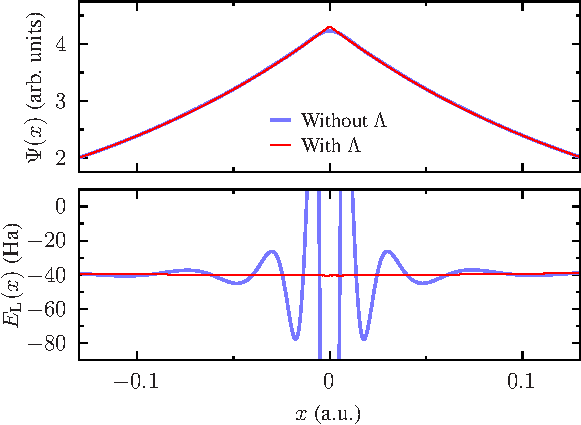
\includegraphics[width=0.8\columnwidth]{figures/optimisation/Fig/cusp-term-eps-converted-to}
    \caption{\gls{HF} wave function value and local energy as a function of the $x$ coordinate of an electron in a carbon atom as it crosses the nucleus at $x=0$, both with and without the $\Lambda$ cusp-correcting Jastrow factor term. This is in the \vdz basis.}
    \label{fig:cusp-term}
\end{figure}

For the calculations in this chapter, we use a total of $44$ optimisable Jastrow factor parameters for the atoms and homonuclear dimers, and $88$ parameters for CN. We keep the $L_v$, $L_\chi$ and $L_f$ cutoff lengths fixed at $4.5$, $4$, and $4$, for simplicity.

\section{Optimisation Strategy}

We optimise $J$ using \gls{VMC}.

\todo{...}

\subsection{Choosing an Appropriate Sample Size}

\todo{...}

\section{Results}
\todo{mention details about integration will be in a separate chapter}
\todo{mention we use a walker number extrapolation already described in another dissertation (cite Muhammedreza)}
\todo{...}

\subsection{Neglecting Three-Body Excitations}

\todo{...}
\todo{mention Pauli exclusion principle as an argument for why this is a valid approximation (maybe use a figure?)}

\subsection{Basis Set Convergence}

\todo{...}

\section{Conclusion and Outlook}
\todo{mention this is the way we now optimise Jastrow factors, but there is an important extension to the no-3-body approximation, xTC. Briefly describe.}
\todo{...}

\subsection{The xTC Approximation}

\todo{...}

\label{sec:xtc}
